\section{Implementation}
%%%%%%%%%%%% MID WAY AGENDA %%%%%%%%%%%%%%
%\begin{frame}<beamer>
%\frametitle{Thomas Holm Pilgaard}
%\tableofcontents[currentsection]
%\end{frame}
%%%%%%%%%%%% MID WAY AGENDA %%%%%%%%%%%%%%

\begin{frame}{Implementation}{Simulink}
\begin{itemize}
\item<1-> MPC control strategy for 24 hours
\item<1-> At each hour:
	 	\begin{itemize}
	 	\item<1-> Iterate $\hat{d}[k]$ and $c_p [k]$
	 	\item<1-> Measurement on the states 
	 	\item<1-> Apply control input $\pmb{\hat{U}_{Hp}}(1,1)$
	 	\end{itemize}
\end{itemize}

\begin{figure}[H]
\centering
\begin{tikzpicture} [scale=0.67,transform shape]

\draw  (10,2) rectangle (6,0);
\node at (8,1) {Model};
\node at (9.7,1.7) {$\hat{y}$};
\node at (9.7, 0.3) {$\hat{x}$};
\node at (6.3, 1.7) {$\hat{d}$};
\node at (6.3, 0.3) {$\hat{u}$};
\draw[-triangle 60] (10, 1.7) -- (11, 1.7);

\draw[-triangle 60] (10, 0.3) -- (11, 0.3) -- (11,-3) -- (9,-3);

\draw  (9,-2) rectangle (7,-4);
\node at (8,-3) {MPC};
\node at (6.5,-2.55) {$\pmb{\hat{u}_{Hp}}$};
\draw  (7,-3) -- (6,-3);
\draw (6,-3.3) rectangle (4,-2.7);
\draw (8.5,2) rectangle (7.9,1.5);
\node at (8.2,1.8) {$T_s$};

\draw  (5.8,-3.3) -- (5.8,-2.7);
\draw  (5.6,-3.3) -- (5.6,-2.7);
\draw  (5.4,-3.3) -- (5.4,-2.7);
\draw  (5.2,-3.3) -- (5.2,-2.7);
\draw  (5.0,-3.3) -- (5.0,-2.7);
\draw  (4.8,-3.3) -- (4.8,-2.7);
\draw  (4.6,-3.3) -- (4.6,-2.7);
\draw  (4.4,-3.3) -- (4.4,-2.7);
\draw  (4.2,-3.3) -- (4.2,-2.7);
\fill[ForestGreen] (4.18,-3.29) rectangle(4.01,-2.71);
\draw[-triangle 60] (4, -3) -- (3, -3) -- (3,0.3) -- (6,0.3);
\node at (3.9,-1.5) {$\pmb{\hat{u}_{Hp}}(1,1)$};
\draw[-triangle 60] (5,1.7)--(6,1.7);

 
    \draw (0,1.7) -- (4.3,1.7);
    \node [font=\large] at (4.3,1.5) {t};
    \draw (0,2.4)node[left,font=\large] {$\hat{OD}$} -- (0,1.0);
    % \draw (0.2,-1)node[left,font=\tiny] {$y=-1$} -- (11.8,-1); 
    % \foreach \x in {0,0.5,...,12}{
    % \draw (\x,-0.2)node [below,font=\tiny,] {\x} -- (\x,0.2) ;
    % }
    \draw[ thick, red] (0,1.7) sin (0.7,2.4);    %% the real business in this line
    \draw[ thick, red] (0.7,2.4) cos (1.4,1.7);    %% the real business in this line
    \draw[ thick, red] (1.4,1.7) sin (2.1,0.9);    %% the real business in this line
    \draw[ thick, red] (2.1,0.9) cos (2.8,1.7);    %% the real business in this line
    \draw[ thick, red] (2.8,1.7)  sin (3.5,2.4);    %% the real business in this line
    \draw[ thick, red] (3.5,2.4) cos (4.2,1.7);    %% the real business in this line
    % \draw[ultra thick, red] (9,0) sin (10,-1);    %% the real business in this line
    % \draw[ultra thick, blue] (10,-1) cos (11,0);    %% the real business in this line

\end{tikzpicture}%


 
\end{figure}

\end{frame}



% \begin{frame}{Implementation}{}
% % \begin{figure}[H]
% % \centering
% % \includegraphics[width=1\textwidth]{Sections/Billeder/result_1020_4050}
% % \end{figure}
% \end{frame}

\section{Results}

\begin{frame}{Results}{New results}
% \begin{figure}[H]
% \centering
% \includegraphics[width=1\textwidth]{Sections/Billeder/result_1030_1050}
% \end{figure}

\begin{figure}[H]
   \centering
    % This file was created by matlab2tikz.
%
%The latest updates can be retrieved from
%  http://www.mathworks.com/matlabcentral/fileexchange/22022-matlab2tikz-matlab2tikz
%where you can also make suggestions and rate matlab2tikz.
%
\definecolor{mycolor1}{rgb}{0.00000,0.44700,0.74100}%
%
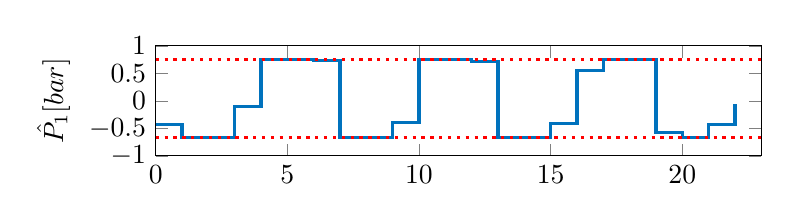
\begin{tikzpicture}

\begin{axis}[%
width=3.028in,
height=0.55in,at={(1.011in,4.137in)},
scale only axis,
xmin=0,
xmax=23,
ymin=-1,
ymax=1,
ylabel={$\hat{P_1}[bar]$},
%xmajorgrids,
%ymajorgrids,
axis background/.style={fill=white},
title style={font=\bfseries},
%title={$\text{u}_{\text{hp1}}\text{[k=0]}$}
]
\addplot[const plot,color=mycolor1,solid,forget plot,very thick] plot table[row sep=crcr] {%
0	-0.433446931217239\\
1	-0.669999999998947\\
2	-0.669999999997713\\
3	-0.104236955958482\\
4	0.749999999997401\\
5	0.749999999998619\\
6	0.727077455814283\\
7	-0.669999999999055\\
8	-0.66999999999925\\
9	-0.395725243988171\\
10	0.749999999988271\\
11	0.749999999998319\\
12	0.717572940373614\\
13	-0.669999999998221\\
14	-0.669999999999149\\
15	-0.409583761852645\\
16	0.548034702463677\\
17	0.749999999998184\\
18	0.74999999999883\\
19	-0.576396407197271\\
20	-0.669999999998877\\
21	-0.425048538821507\\
22	-0.0640667111129486\\
};
\addplot[const plot,color=red,dotted,very thick] plot table[row sep=crcr] {%
0	0.75\\
24	0.75\\
};

\addplot[const plot,color=red,dotted,very thick] plot table[row sep=crcr] {%
0	-0.67\\
24	-0.67\\
};

\end{axis}
\end{tikzpicture}


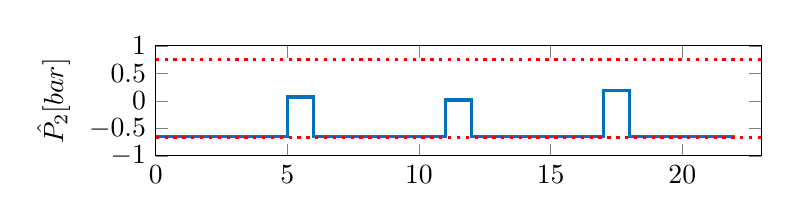
\begin{tikzpicture}

\begin{axis}[%
width=3.028in,
height=0.55in,
at={(1.011in,2.39in)},
scale only axis,
xmin=0,
xmax=23,
ymin=-1,
ymax=1,
%xmajorgrids,
%ymajorgrids,
ylabel={$\hat{P_2}[bar]$},
axis background/.style={fill=white},
title style={font=\bfseries},
%title={$\text{u}_{\text{hp2}}\text{[k=0]}$}
]
\addplot[const plot,color=mycolor1,solid,forget plot,very thick] plot table[row sep=crcr] {%
0	-0.649999999999008\\
1	-0.649999999999539\\
2	-0.649999999999527\\
3	-0.64999999999887\\
4	-0.649999999994262\\
5	0.0667700518106753\\
6	-0.649999999998485\\
7	-0.649999999999511\\
8	-0.649999999999588\\
9	-0.649999999999157\\
10	-0.649999999997306\\
11	0.0160826405819198\\
12	-0.649999999996155\\
13	-0.64999999999941\\
14	-0.64999999999958\\
15	-0.649999999999219\\
16	-0.649999999998156\\
17	0.189015571020597\\
18	-0.649999999956971\\
19	-0.649999999999335\\
20	-0.649999999999555\\
21	-0.649999999999218\\
22	-0.649999999998207\\
};
\addplot[const plot,color=red,dotted,very thick] plot table[row sep=crcr] {%
0	0.75\\
24	0.75\\
};

\addplot[const plot,color=red,dotted,very thick] plot table[row sep=crcr] {%
0	-0.67\\
24	-0.67\\
};
\end{axis}
\end{tikzpicture}

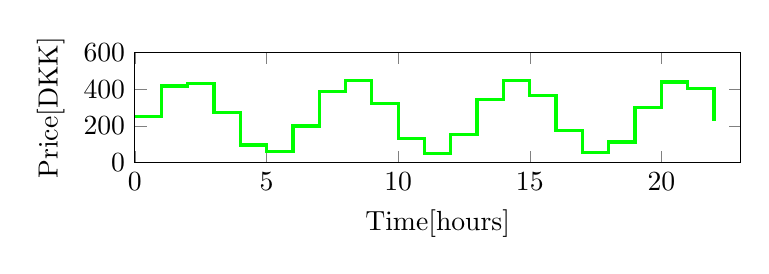
\begin{tikzpicture}

\begin{axis}[%
width=3.028in,
height=0.55in,
at={(1.011in,0.642in)},
scale only axis,
xmin=0,
xmax=23,
xlabel={Time[hours]},
ymin=0,
ymax=600,
%xmajorgrids,
%ymajorgrids,
ylabel={Price[DKK]},
axis background/.style={fill=white},
title style={font=\bfseries},
]
\addplot[const plot,color=green,solid,forget plot,very thick] plot table[row sep=crcr] {%
0	250\\
1	418.857649358291\\
2	430.978019589665\\
3	275.110723996831\\
4	95.9351176989303\\
5	59.7658279797972\\
6	200.175962602534\\
7	386.833833626164\\
8	446.479615730073\\
9	323.748819156816\\
10	132.562792409559\\
11	50.3844917318038\\
12	153.493572208496\\
13	346.181981592006\\
14	449.592219965457\\
15	367.736693884804\\
16	176.595452155304\\
17	53.5898806097876\\
18	112.896379753435\\
19	299.465389524004\\
20	440.119567515206\\
21	404.300699515516\\
22	225.256624358491\\
};
\end{axis}
\end{tikzpicture}%
\end{figure}

\end{frame}


\section{Discussion}
\begin{frame}{Discussion}{}

\begin{itemize}
	\item<1->The next step
	\begin{itemize}
	 \item<1-> Solving implementation problems  
	 \item<1-> Comparing the results with the real system
	\end{itemize}
\end{itemize}

\begin{itemize}
\item<2-> Future research
	 \begin{itemize}
	 \item<2-> Using a nonlinear model for parameter estimation 
	 \item<2-> Adaptive control
	 \end{itemize}
\end{itemize}

\end{frame}
